\chapter{\textbf{Desarrollo}}

\thispagestyle{empty}

En el presente capítulo se detalla la planificación siguiendo la metodología Turpial Agile Unified Process (TAUP). Adicionalmente, se describe la evolución del proyecto y sus dificultades, así como las actividades realizadas que llevaron a cumplir los objetivos planteados y logros adicionales.

\section{Fase de concepción}

En esta sección se detallan las funcionalidades de los módulos Principal (\textit{Core}) y Estadísticas de la librería Auditorías Turpial según los requerimientos del cliente; y se muestra el diseño de la solución y  planteamiento de la arquitectura. También, se elaboran los documentos según TAUP y se definen las tecnologías necesarias para el desarrollo del proyecto. Este proceso abarcó las primeras cuatro semanas de la pasantía.

\subsection{Análisis de requerimientos}

Antes de tomar alguna decisión de implementación, fue necesario establecer cuál es la tecnología a la que va dirigida el producto final y cuáles son las funcionalidades mínimas que debe poseer. En primer lugar, se decidió que se desarrollaría una librería en Django, para Django, ya que la empresa suele utilizar este herramienta en sus aplicaciones; y utilizaría una base de datos relacional, en particular PostgreSQL, MySQL o SQLite porque se integran fácilmente al \textit{framework} . \\

En segundo lugar, se determinaron las Historias de Usuario (HU). La librería consta de tres módulos: \textit{Core}, Estadísticas y Reportes. El líder del proyecto se encargó de las HU correspondientes al módulo Principal y el pasante realizó el levantamiento de requerimientos del módulo de Estadísticas (ver apéndice C) según las necesidades del cliente. Adicionalmente, elaboró los documentos correspondientes, Documento de Requerimientos y \textit{Release Plan} siguiendo las plantillas de la empresa. \\

En este caso en particular, el rol del cliente lo interpretó la empresa misma, puesto que el producto será ofrecido como un servicio a clientes externos. El rol de \textit{product owner} lo desempeñó el tutor industrial para gestionar el desarrollo de la pasantía. \\

Para escribir las HU, es indispensable contar con el actor que ejecuta alguna acción específica, por lo que se distinguieron dos tipos de usuarios:

\begin{itemize}
    \item El programador, quien descargará la librería y la incluirá en la aplicación de Django que está desarrollando.
    \item Los “usuarios” finales, quienes utilizarán la aplicación en donde se instale la librería y la interfaz gráfica provista.
\end{itemize}

En líneas generales, el módulo \textit{Core} debe contar con las siguientes características:

\begin{itemize}
    \item Seleccionar cuál modelo (tabla) es auditable.
    \item Registrar el autor, acción, fecha, estado anterior y estado actual de una instancia particular en formato JSON. Las acciones auditables son: Crear, Actualizar y Eliminar.
    \item Listar todas las operaciones, filtrarlas y ordenarlas.
    \item Restringir el acceso del personal no autorizado a los listados.
    \item Proveer etiquetas personalizadas para las plantillas de los listados que faciliten la inclusión de los mismos.
\end{itemize}

El módulo de Estadísticas debe proveer el cálculo del total de auditorías, cantidad de modelos auditables, porcentaje de cobertura, porcentaje de crecimiento de los datos, promedio por día, mínimo y máximo. Dichos resultados pueden estar filtrados por un rango de tiempo, por acción, por autor y por modelo. Asimismo, debe contar con facilidades para incluir los gráficos que representen los cálculos mencionados anteriormente. \\

El módulo de Reportes ofrece la posibilidad de generar archivos sobre los listados en diversos formatos (CSV y PDF) y personalizar su apariencia con opciones como modificar los márgenes, espacios, incluir el nombre y logo del sistema, entre otros. Adicionalmente, la librería debe ser mantenible, eficiente, simple, confiable, escalable y fácil de integrar y configurar.\\

Por otro lado, es indispensable que se instalen automáticamente las dependencias de la librería en el sistema que la utilice para facilitar su uso y evitar errores. También, se requiere que la librería se actualice mediante el uso de una herramienta de integración continua. \\

En esta pasantía se abarcarán las funcionalidades correspondientes a la selección del modelo auditable, registro de traza de auditoría y listados (sin filtros ni ordenamiento) del módulo \textit{Core} y completamente el módulo de Estadísticas con sus respectivas pruebas automatizadas. También se incluye la instalación y configuración del sistema de integración continua. El módulo de Reportes está fuera del alcance.

\subsection{Adaptación de la metodología a la pasantía}

En el capítulo anterior se explicó la metodología TAUP, sin embargo, dependiendo del proyecto que se desea desarrollar, se pueden realizar algunas modificaciones que mejoren la dinámica y la velocidad del equipo o porque el cliente así lo requiera.\\

Se ideó un código compuesto por una letra y un número que facilita referenciar las HU. La letra representa el módulo a la que pertenece, \textit{Core} o Estadísticas, y el número denota el orden en que fue concebida. Adicionalmente, se utilizó una modificación  para las escalas de prioridad y riesgo, que está conformada por tres valores: alta, media y baja. Para más información sobre las HU desarrolladas, leer el Apéndice C.\\

Por otro lado, se agregaron nuevos criterios a la \textit{Definition of Ready}, con lo que se tiene lo siguiente:

\begin{itemize}
    \item Debe ubicarse dentro de uno de los módulos del proyecto.
    \item Debe de tener asignado una prioridad por el cliente.
    \item Debe de tener asignado un riesgo por el equipo de desarrollo.
    \item Debe de tener asignado su respectivo puntaje.
    \item (Opcional pero deseado) Debe de tener una breve descripción, aclaratoria o criterio adicional según sea el caso.
\end{itemize}

Asimismo, se amplió la \textit{Definition of Done} para agregar las pruebas automatizadas de cada HU. Posee los siguientes estatutos:

\begin{itemize}
    \item Debe realizarse la codificación respectiva
    \item El código generado debe estar debidamente documentado para facilidad de programador
    \item Debe de realizarse la documentación respectiva (de ser necesaria) de todos los aspectos de configuración asociados al desarrollo y buen funcionamiento de la historia de usuario.
    \item Deben realizarse pruebas automatizadas a la codificación generada.
    \item Debe presentarse la nueva funcionalidad al cliente.
    \item Debe estar disponible en el repositorio.
\end{itemize}

\subsection{Arquitectura propuesta del sistema}

El planteamiento inicial (Figura 6.1) consistía en desarrollar cada módulo de la librería en una aplicación de Django distinta, las cuales se instalarían por separado en el sistema, el cual será referido como “Host” para simplificar la notación. Los módulos de Estadística y Reportes serían ofrecidos como microservicios dependientes del módulo principal pero independientes entre ellos, de manera que si alguno falla, el otro no sea afectado.\\

\begin{figure}
\centering
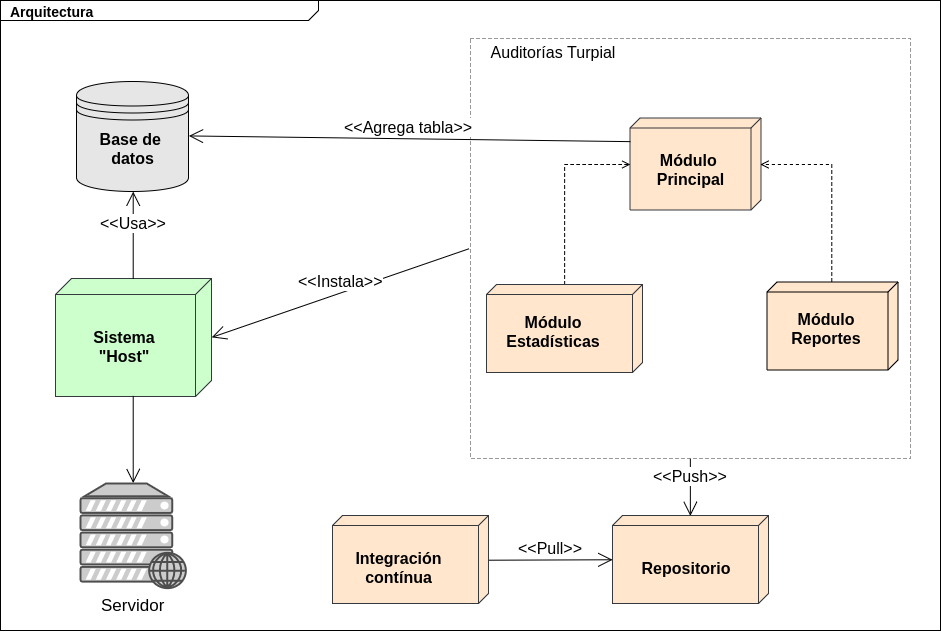
\includegraphics[width=\textwidth]{Diagrama_Arquitectura.png}
\caption{Arquitectura de la librería Auditorías Turpial}
\label{fig:figure6.1}
\end{figure}

Se decidió que el módulo Principal agregaría una nueva tabla en la base de datos ya existente del “Host” en la que mantendrá la información acerca de las auditorías y los otros módulos podrían leerla para procesarla y mostrarla como sea  pertinente.\\

No obstante, la arquitectura mostrada en la figura 6.1 sufrió modificaciones durante el desarrollo  el proyecto para simplificarla. En lugar de crear tres aplicaciones, una para cada módulo, se separó Auditorías Turpial en dos: \textit{backend} y \textit{frontend}. En la sección que explica la fase de construcción se ofrecerán mayores detalles de estos cambios y sus razones. \\

\begin{figure}
\centering
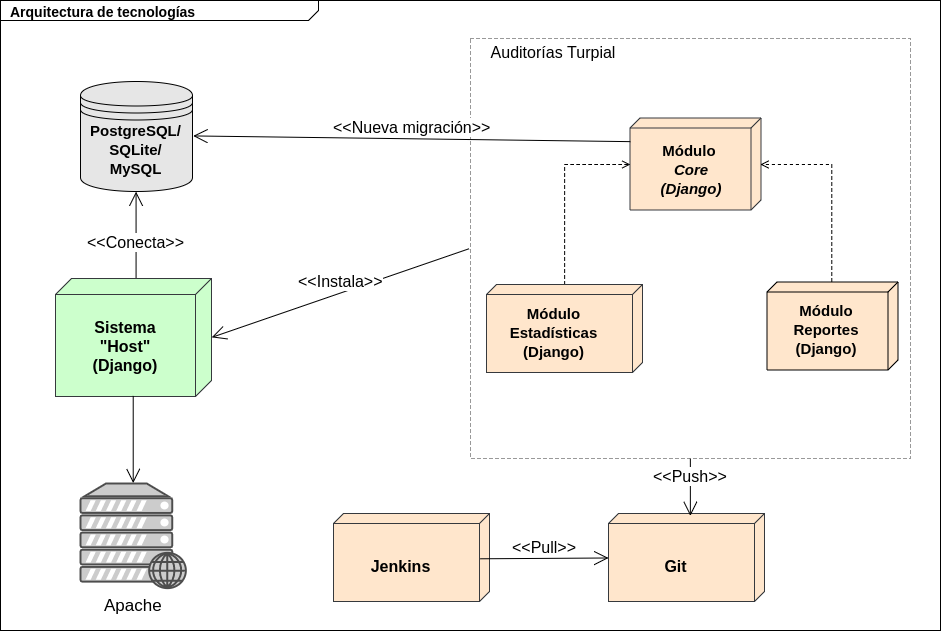
\includegraphics[width=\textwidth]{Diagrama_Tecnologias.png}
\caption{Arquitectura de tecnologías a utilizar}
\label{fig:figure6.2}
\end{figure}

En la figura 6.2 se muestran las tecnologías a utilizar en el proyecto. Como se mencionó anteriormente, se utilizará Django para el desarrollo. Como herramienta de control de versiones se utilizará Git y para automatizar la integración continua se usará Jenkins. El sistema “Host” será un proyecto de la empresa que utilizará como servidor Web, Apache y una base de datos relacional.

\subsection{Diseño del módulo \textit{Core}}

Uno de los problemas más significativos que la empresa encuentra en otras extensiones de Django disponibles, es el hecho de que el registro de auditoría se guarda a nivel de la vista y es responsabilidad del programador colocar el código para esta funcionalidad. Esto da cabida a que se olvide colocar en alguna de las vistas correspondientes a algún modelo, por lo que podría no guardarse todos los tipos de operaciones. \\

La librería Auditorías Turpial pretende evitar este problema guardando el registro de auditoría cada vez que ocurre alguna operación sobre el modelo a través del uso de las \textit{signals} que ofrece el \textit{framework} . Éstas, necesariamente deben distinguir entre un modelo auditable y uno que no lo es. Para esto, se contempló el uso de un \textit{mixin} que pueda ser heredado por cualquier modelo y así proveer todas las funcionalidades mencionadas. \\

Por otro lado, se desea incluir en las auditorías el usuario que realizó la acción. La solución mencionada anteriormente no es suficiente para lograr esto, puesto que a nivel de modelos no se posee información sobre el \textit{request} y no se puede saber qué usuario está en sesión. Por esta razón, se planteó agregar otro \textit{mixin} a nivel de vistas que completara la información antes de guardarla en la base de datos. Sería responsabilidad del programador heredarlo en todas las vistas cuyos modelos mantienen un historial de transacciones.\\

Django posee mecanismos para traducir los modelos a otro formato con una estructura bien definida, más conocidos como \textit{serializers}. En particular, posee maneras de convertirlos a JSON, por lo que se decidió utilizar dicha funcionalidad para cumplir con el requisito de mostrar los cambios en los valores de los campos del modelo auditable en este formato.\\

En cuanto a los listados, se acordó utilizar Datatables para mostrarlos como una tabla que se pueda ordenar y filtrar fácilmente. Este \textit{plugin} puede manejar aproximadamente 10000 filas en sus tablas procesándolas del lado del cliente. Sin embargo, las auditorías serán potencialmente millones de registros, es por esta razón se debe realizar el procesamiento del lado del servidor. \\

Para la autenticación se consideró utilizar una tabla de usuarios propia con su respectiva permisología, con la intención de que no interfiriera con la del sistema “Host”, sin embargo, esto no fue posible. Se profundizará esta explicación de esta decisión en la fase de desarrollo del presente capítulo.

\subsection{Diseño del módulo de estadísticas}

Uno de los requisitos mínimos con el que debe contar el módulo de Estadísticas es exponer un conjunto de gráficas que permitan visualizar e interpretar fácilmente los resultados de los cálculos de las auditorías. Para esto, se investigaron dos librerías de JavaScript: Amcharts y Charts.js. En la siguiente tabla se muestran las características principales:\\

\begin{table}[h]
\centering
\caption{Comparación de Amcharts vs Charts.js}
\label{tabla:6.2}
\begin{tabular}{| p{\textwidth/4} | p{\textwidth/3} | p{\textwidth/3} |}
\hline
                                              & \textbf{Amcharts}                                                       & \textbf{Chart.js}                                            \\ \hline
\textbf{Código abierto}                       & Sí.                                                                     & Sí.                                                          \\ \hline
\textbf{Tipos de gráficos}                    & Línea, área, barras, torta, \textit{Scatter}, Gantt, Radar, de vela, entre otras & Línea, área, barras, torta, \textit{Scatter}, Radar, entre otras.     \\ \hline
\textbf{Tecnología para mostrar los gráfico}  & SVG                                                                     & HTML5 Canvas                                                 \\ \hline
\textbf{Líneas de tendencia}                  & Sí.                                                                     & Sí.                                                          \\ \hline
\textbf{Responsive}                           & Sí.                                                                     & Sí.                                                          \\ \hline
\textbf{Exportar los datos}                   & Sí, mediante un \textit{plugin}.                                                 & No.                                                          \\ \hline
\textbf{Zoom}                                 & Sí.                                                                     & Sí. Utilizando un \textit{plugin}.                                    \\ \hline
\textbf{Soporta múltiples lenguajes}          & Sí                                                                      & No.                                                          \\ \hline
\textbf{Librería integrada con Django}        & No.                                                                     & Sí.                                                          \\ \hline
\textbf{Manejo de grandes volúmenes de datos} & Sí.                                                                     & No. Según opiniones de los usuarios, disminuye el desempeño. \\ \hline
\end{tabular}
\end{table}


Como los desarrolladores de Turpial Development son los principales usuarios de este proyecto, el pasante investigó si existía alguna librería que utilicen usualmente. En la empresa han utilizado varias, incluyendo las dos presentadas anteriormente, por lo que no tienen una preferencia en este sentido. \\

Debido a que la cantidad de registros de auditorías pueden crecer rápidamente, es necesario escoger una librería de gráficos que maneje adecuadamente grandes volúmenes de datos, por lo que se decidió utilizar Amcharts. Otra característica que inclina la balanza a favor de esta solución, es el hecho de que posee un \textit{plugin} que permite exportar datos a un archivo CSV o PDF, una funcionalidad que se compenetra bien con el módulo de Reportes. \\

Aunque Charts.js posee una extensión de Django para facilitar la creación de los gráficos a través de las vistas, este proyecto requiere una lógica muy específica para entregar el conjunto de datos que se utilizará para mostrarlos. Por esta razón, es mejor tener total control sobre su implementación. \\

Los cálculos estadísticos serán entregados a la plantilla a través de una vista que incluirá el formulario de los filtros y la manipulación de los datos para crear los gráficos pertinentes y según los requiera la librería escogida.

\subsection{Propuesta para la integración continua}

Dado que en la empresa no existe precedente sobre el uso de una herramienta automatizada para integrar el código de manera continua, se le otorgó al pasante la libertad de escoger entre dos herramientas sugeridas por el líder del proyecto: Jenkins o Fabric. Para decidir cuál herramienta se adecuaba más al proyecto y a las necesidades de la empresa, fue indispensable que el pasante investigara las opciones en profundidad, sus fortalezas, limitaciones y recomendaciones de la comunidad. A continuación se muestra una comparación entre ellas: \\

\begin{table}[h]
\centering
\caption{Comparación de Jenkins vs Fabric.}
\label{tabla:6.1}
\begin{tabular}{| p{\textwidth/4} | p{\textwidth/3} | p{\textwidth/3} |}
\hline
                                                 & \textbf{Jenkins}                                                                                                                                   & \textbf{Fabric}                                                                                                                                              \\ \hline
\textbf{Descripción}                             & Un servidor de automatización que puede ser utilizado para automatizar cualquier clase de tarea cómo construir, probar y desplegar software        & Es una librería y una herramienta de línea de comandos para coordinar el uso de SSH para despliegues de aplicaciones o tareas de sistemas de administración. \\ \hline
\textbf{Código abierto}                          & Sí.                                                                                                                                                & Sí.                                                                                                                                                          \\ \hline
\textbf{Lenguaje}                                & Escrito en Java                                                                                                                                    & Escrito en Python                                                                                                                                            \\ \hline
\textbf{Extensible}                              & Si. Cuenta con una gran cantidad de \textit{plugins} para ampliar sus funcionalidades básicas y una tienda en donde pueden adquirirse                       & No.                                                                                                                                                          \\ \hline
\textbf{Interfaz gráfica}                        & Sí.                                                                                                                                                & No.                                                                                                                                                          \\ \hline
\textbf{Integración con Gitlab}                  & Sí.                                                                                                                                                & No                                                                                                                                                           \\ \hline
\textbf{Ejecutar un script}                      & Sí.                                                                                                                                                & Sí.                                                                                                                                                          \\ \hline
\textbf{Empaquetamiento y despliegue programado} & Si. Se puede configurar un horario para ejecutar algún script que contenga todas las instrucciones para empaquetar, probar y desplegar el sistema. & No. Se debe ejecutar el archivo de configuración a través de la consola.                                                                                     \\ \hline
\textbf{Observaciones}                           & Altamente recomendado por la comunidad.Puede generar reportes de las pruebas ejecutadas.                                                           & Fácil de aprender, de configurar y de instalar.                                                                                                              \\ \hline
\end{tabular}
\end{table}


Considerando las características que posee cada herramienta, se decidió
utilizar Jenkins puesto que se pueden ejecutar \textit{scripts} de manera
programada, generar reportes, observar el estado del despliegue de varios
proyectos e incluso integrarlo con Gitlab, un servicio Web de control de
versiones y desarrollo de \textit{software} colaborativo basado en Git que es
utilizado por la empresa. \\

Si bien Fabric es más simple, no es realmente un servidor para integración
continua, se asemeja más a \textit{scripts} que permiten automatizar tareas y
se requiere de una herramienta suficientemente general que pueda ser usado
tanto en la pasantía como en otros proyectos de la empresa.

\subsection{Plan de pruebas}

Para verificar que cada funcionalidad posea el comportamiento esperado, se realizaron pruebas de manera automatizada utilizando Pytest. Más específicamente, se llevaron a cabo pruebas unitarias, de regresión y de integración. \\

Adicionalmente, se convino que uno de los criterios de aceptación de las HU era validar el producto con el cliente para asegurar el cumplimiento de las reglas de negocio y que el producto desarrollado cumple los estándares. A esto se le conoce como pruebas de aceptación y fueron realizadas en cada cierre de \textit{Sprint}.\\

Como el proyecto en cuestión es una librería, no puede funcionar por sí sola, sino que necesita instalarse en otro. Para esto, se creó una aplicación sencilla en Django y se instaló la librería en él. En cada \textit{Sprint}, se constató que el programador pueda usar cada funcionalidad desarrollada  sin ningún inconveniente. Este mismo proyecto, se utilizó para mostrar los avances al cliente. \\

En la fase de transición, se planificó que se realizaran pruebas en una aplicación desarrollada para uso interno de la empresa, llamado Turpial Team. No obstante, debido a que aún se encuentra en desarrollo no está disponible actualmente. Se optó por utilizar otro proyecto de uso interno de Turpial Development, llamado Turpial Calendar. Esta aplicación sirve para planificar eventos de la empresa y enviar notificaciones. Esta decisión no afecta de ninguna manera la pasantía ya que la librería debe poder ser instalada en cualquier proyecto con las características mencionadas en la sección de requerimientos. \\

En el apéndice E se encuentra el documento de  Plan de Pruebas creado para la empresa, para ofrecer más detalle de los explicado en esta sección.\\

\subsection{Planificación del desarrollo del proyecto}

Luego de finalizar el proceso de investigación, aclarar los requerimientos y determinar las HU, se procedió a planificar la fase de construcción del proyecto. Para ello, se tomó en cuenta la prioridad, precedencia y puntaje de cada HU para determinar el orden. Se decidió iniciar con las HU relacionadas con el \textit{Core} y la instalación de la librería.\\

Se planificaron ocho \textit{Sprints} con una duración de dos semanas laborales (diez días) cada uno. Estos \textit{Sprints} abarcan la fase de construcción del módulo \textit{Core} y Estadísticas de Auditorías Turpial, así como la fase de transición.

\section{Fase de construcción}

Una vez culminada la fase de concepción, se procedió con la instalación del ambiente de desarrollo e implementación de los módulos que abarca la pasantía. También, se incluyen las pruebas pertinentes para cada funcionalidad desarrollada según indica el Plan de Pruebas.

\subsection{Construcción del módulo \textit{Core}}

En esta sección se describe el proceso para desarrollar cada HU relacionada con el módulo \textit{Core}, los problemas encontrados y sus soluciones. También se explica el nuevo diseño de la arquitectura y las pruebas efectuadas.

\subsubsection{Preparación del ambiente de desarrollo}

Antes de iniciar con la implementación de la librería, se instalaron y configuraron todas las herramientas necesarias para esto. En primer lugar, se instaló Python 2.7 y luego PIP. Se instaló el \textit{plugin} de Python, Virtualenv, el cual permitió configurar el ambiente virtual. Este, se utilizó para instalar los requerimientos de la librería, en particular, Django 1.10 y Pytest 3.2. Estos, se registraron en el archivo “requirements.txt” para facilitar futuras instalaciones y determinar las dependencias de la librería. Luego, se procedió a crear la aplicación de Django y la estructura del módulo \textit{Core}.

\subsubsection{Estructura de la tabla de auditorías}

Para registrar apropiadamente la información de la auditoría como fue establecida en la fase anterior, se creó un modelo en Django cuyo nombre es “AuditableAction". Este se agregará como una tabla adicional en la base de datos del sistema “Host" y posee los siguientes campos:\\

\begin{table}[h]
\centering
\caption{Modelo de datos de la tabla “AuditableAction"}
\label{tabla:1.3}
\begin{tabular}{| p{0.20\textwidth} | p{0.25\textwidth} | p{0.45\textwidth} |}
\hline
\textbf{Nombre del campo} & \textbf{Tipo de dato (Django)}                              & \textbf{Descripción}                                                                                                                                                                   \\ \hline
ID                        & \textit{AutoField}                                 & Identificador del registro auditable. Entero de 32 bits. Los valores van desde -2147483648 a 2147483647.                      \\ \hline
author                    & \textit{ForeignKey}                                         & Referencia al usuario que realizó la acción.                                                                                                                                           \\ \hline
action                    & \textit{CharField}. Limitado a las opciones: CREATED,
UPDATED, DELETED. & El tipo de acción efectuada sobre un modelo auditable.                                                                                                                                 \\ \hline
datetime            & \textit{DateTimeField} & Fecha en la que se registró la acción.\\ \hline
model\_name               & \textit{CharField}                                 & Nombre del modelo auditable.  \\ \hline
model\_json\_old          & \textit{JSONField}                                 & Antiguo valor. Un JSON que representa el valor que tenía el registro que se ve afectado por la operación. En caso de que la acción sea “creado", el JSON representará el objeto vacío. \\ \hline
model\_json\_new          & \textit{JSONField}                                 & Nuevo valor. Un JSON que representa el valor que tiene el registro que se ve afectado por la operación. En caso de que la acción sea “eliminado", el JSON representará el objeto vacío \\ \hline
\end{tabular}

\end{table}


En cuanto a los campos tipo JSON, se utilizó la \textit{plugin} de Django, Jsonfield, que provee todos los validadores necesarios para que el campo de sea considerado un JSON, y así, mantener la integridad de la base de datos. Adicionalmente, este \textit{plugin} puede hacer uso del campo JSON que posee nativamente PostgreSQL; en el resto de los manejadores, se representa como un campo de texto.

\subsubsection{Selección de un  modelo auditable}

Para que un programador pueda escoger qué modelo es auditable y cuál no, se creó un \textit{mixin} a nivel de modelos, llamado "AuditableMixin". Este permite heredar el comportamiento necesario para registrar las auditorías en la base de datos.

\subsubsection{Registro de una acción auditable}

Como bien se ha dicho antes, Django posee \textit{signals} que son detonadas por diferentes eventos; dos de ellos están relacionados con la creación y actualización de objetos, “pre\_save” y “post\_save”. Estas señales se activan antes de guardar un objeto en la base de datos y después, respectivamente; bien sea para crearlo o actualizarlo. Cada una de ellas posee información sobre la instancia que será guardada en la base de datos y el modelo que envía la señal (\textit{sender}). El \textit{sender} es de gran utilidad puesto que permite determinar cuál es su clase, y así auditar solo los modelos que sean una subclase del "AuditableMixin" definido anteriormente.\\

En principio, se optó por hacer un manejador para la señal “pre\_save” debido a que, antes de guardar en base de datos, se puede obtener tanto el valor actual de la instancia como el que tendrá. Desafortunadamente, esta solución no asegura que se almacene la instancia a auditar en la base de datos, pero sí la traza de auditoría. Podría ocurrir algún error justo en medio de estas dos operaciones lo que generaría problemas de consistencia.\\

Utilizar la señal “post\_save” tampoco fue una opción, ya que no se podía obtener el valor del registro anterior, lo cual es de suma importancia para comparar los cambios ocurridos. \\

Motivado por esto, se decidió sobreescribir el método “save()”, con lo que se puede realizar el procesamiento para capturar el valor anterior, guardar el objeto auditable y generar la auditoría. Se distingue el tipo de acción si la instancia posee o no una clave primaria; si no la posee se está creando.\\

El primer inconveniente encontrado con esta solución es el hecho de que, al cargar la base de datos con un \textit{Fixture}, el \textit{framework} no utiliza “save()”. Asume que los datos dentro del archivo son íntegros y los inserta, activando las señales correspondiente. El segundo, es que este comportamiento se replica con las inserciones y actualizaciones masivas, “bulk\_create” “bulk\_update”. Los mencionados métodos se traducen directamente a sentencias de SQL, por lo que tampoco activan \textit{signals}.  En la documentación de la librería se explican estos problemas y esperan ser corregidos en una próxima versión.\\

Con respecto a la acción DELETE, no hubo mayores contratiempos, se utilizó la señal “post\_save”, la cual se activa luego de que se elimina una instancia, dado que no se requiere registrar el valor posterior.\\


\textbf{Relación muchos a muchos} Django cuenta con la facilidad de, a nivel de modelos, crear relaciones muchos-a -muchos sin necesidad de que el programador explícitamente genere la tabla intermedia que los conecta; a través del campo "ManyToManyField". Los cambios ocurridos en ellos, activan una señal llamada “m2m\_changed”, la cual se utilizó para llevar control de los cambios de apuntadores (llaves primaria) hechos. No obstante, fue descartado debido a que el comportamiento natural del \textit{framework} cuando se crea por primera vez el registro, es guardar la instancia sin los cambios en estos campos y luego guardarlos nuevamente.\\

\begin{figure}[h]
\centering
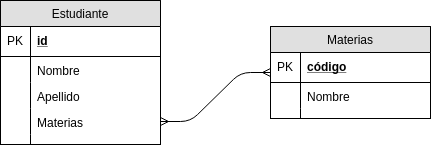
\includegraphics[width=0.6\textwidth]{Estudiante-Materia.png}
\caption{Modelo Entidad-Relación del ejemplo.}
\label{fig:figura6.3}
\end{figure}

Por ejemplo, si se tiene un tabla Estudiante, que tiene una relación muchos-a-muchos con Materias como muestra la figura 6.3, al intentar guardar una instancia de Estudiante con algunas Materias, se sigue el siguiente flujo:\\

\begin{figure}[h]
\centering
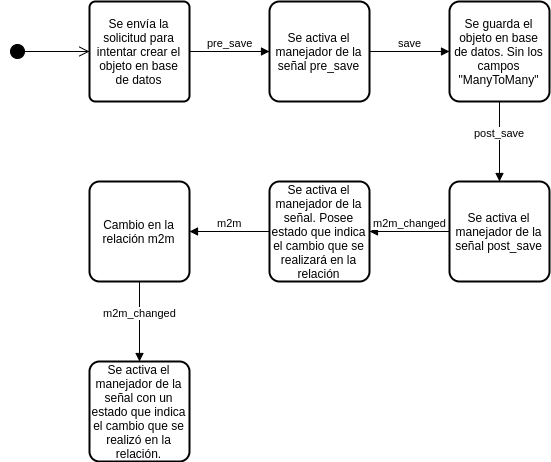
\includegraphics[width=0.8\textwidth]{Signals.png}
\caption{Gráfico de flujo del orden en el que se activan las señales para guardar un cambio en los campos “ManyToManyField”.}
\label{fig:figura6.4}
\end{figure}

Debido al orden en que se activan la señales (figura 6.4), se almacena el objeto en base de datos y luego, cuando cambia el campo "materias", se guarda nuevamente, por lo que era imposible obtener en un sólo registro de auditoría todos los cambios.\\

El pasante propuso al cliente dos opciones: la primera es permitir que se generen dos registros de auditoría, el primero con acción CREATE y el segundo con UPDATE, puesto que en realidad es una actualización. La segunda, es excluir esta relación de la auditoría, es decir, no utilizar “m2m\_changed”.\\

Esta última, fue la escogida por el cliente y se documentó apropiadamente. Si el programador desea llevar auditorías de los cambios ocurridos en casos como estos, puede escribir su propia tabla intermedia para relacionar ambos modelos y utilizar la opción "through" provista por “ManyToManyField” como indica la documentación de Django. Si, esta tabla, hereda el “AuditableMixin” se replica el comportamiento buscado inicialmente al incluir los campos muchos-a-muchos\\

\textbf{\textit{Serializers}}  Como se diseñó en la fase de concepción, se utilizaron los \textit{serializers} provistos por el \textit{framework} para almacenar la estructura completa de la instancia en cuestión, con el formato JSON. Los \textit{serializers} incluyen la clave primaria del objeto, el nombre del modelo y los campos que este contiene.\\

Automáticamente, Django incluye la representación de los campos “ManyToManyField” y al decidir no rastrear los cambios en estos, fue necesario excluirlos explícitamente para evitar inconsistencias y confusiones.\\

\textbf{Inclusión del usuario en la traza de auditoría}  Lo explicado anteriormente funciona perfectamente para registrar la auditoría y verificar los cambios, sin embargo no es suficiente para obtener el usuario, puesto que a nivel de modelos no se cuenta con esta información. Para solucionar esto, se creó otro \textit{mixin} llamado "AuditableMixinView", que inyecta la información del usuario en un campo oculto incluido en el "AuditableMixin". De esta manera, en las \textit{signals} se puede poseer la información del usuario en sesión y todo lo relacionado con él.

\subsubsection{Instalación de la librería utilizando PIP}

Una vez se obtenida una versión suficientemente sólida de la librería, se prosiguió a satisfacer uno de los requerimientos más importantes: que la librería sea capaz de instalarse  utilizando PIP. El pasante debió documentarse al respecto, debido a que existía gran desconocimiento en todo el equipo. En la página web oficial de Django se encuentra un tutorial bastante detallado para construir extensiones el cual sirvió de guía para el proceso. \\

Lo primero que se hizo fue construir un archivo llamado "setup.py", que contiene la información de la librería, el nombre, la versión, los autores, la licencia y los paquetes que requiere, entre otros. En el caso de Auditorías Turpial, el paquete requerido fue Jsonfield.\\

Luego, se creó el archivo "MANIFEST.in" para incluir aquellos archivos que no son detectados automáticamente por el "setup.py" como las plantillas de Django, los estáticos (javascript, css), la licencia, entre otros. \\

Por último, en la cónsola, posicionados en la carpeta en la que se encuentra el achivo “setup.py”, se procede a empaquetar la librería. Una vez culminado este proceso, se tiene un archivo comprimido que se puede utilizar para instalar la librería con PIP.\\

El pasante documentó con gran detalle este proceso para que el resto de los miembros del equipo pudiesen seguir los pasos. Esta documentación está disponible para la empresa, en caso de que deseen crear una nueva librería o actualizar Auditorías Turpial.

\subsubsection{Listados de auditoría}

Culminada toda la construcción de los \textit{mixins}, \textit{signals} e instaladores de la librería, se procedió a implementar la funcionalidad de listados de todas las auditorías registradas en base de datos. Para esta funcionalidad se decidió utilizar el \textit{plugin} de JavaScript, Datatables, que permite integrar de forma fácil y sencilla una tabla a la plantilla. Los listados son procesados en el servidor y tienen paginación, puesto que las auditorías pueden poseer millones de registros. Con esta decisión se evitan dos aspectos relevantes, sobrecargar el navegador de altos volúmenes de contenidos e incrementar el tiempo de espera del usuario para el cargado de los listados.\\

Al usuario presionar alguno de los botones en la plantilla del listado, se realiza una solicitud GET de dicha página utilizando AJAX. De esta manera, se refresca ese componente sin necesidad de recargar completamente la página, lo que mejora la experiencia de usuario.

\subsubsection{Reestructuración de la arquitectura}

Antes de iniciar con la elaboración de los otros módulos de la librería, se notó que la funcionalidad de generar reportes está íntimamente relacionada con los listados de auditoría. Los filtros y el ordenamiento aplicados a los listados, deben aparecer en los CSV y PDF generados. Es por esta razón que, al finalizar el desarrollo de esta HU, el equipo se replanteó la estructura establecida en la fase de concepción.\\

En lugar de crear tres aplicaciones en Django, una para cada módulo, se decidió crear sólo dos, como muestra la figura 6.5. La primera de ellas sería el backend de Auditorías Turpial, que mantiene toda la lógica para registrar las auditorías, explicada en los puntos anteriores; mientras que la segunda tendría los módulos de Reportes y Estadísticas. A esta última  la llamaremos Auditorías Turpial UI (User Interface) y contendrá todo el frontend del proyecto. Las funcionalidades de los listados fueron colocadas en el módulo de Reportes para facilitar la generación de PDF y CSV.

\begin{figure}[h]
\centering
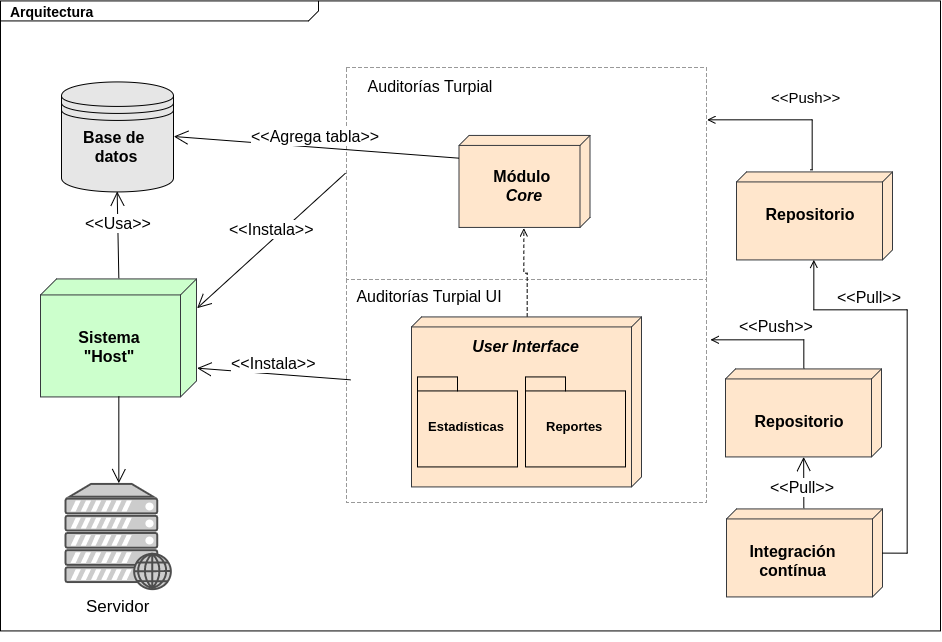
\includegraphics[width=\textwidth]{Diagrama_Arquitectura2.png}
\caption{Arquitectura final de la librería.}
\label{fig:figura6.5}
\end{figure}

Esta reestructuración permite separar la captura de información de la manera en la que se muestra, sin que se vean afectados los beneficios que ofrecen los microservicios. Aunque los módulos de Estadísticas y Reportes se encuentren dentro de la misma aplicación, el programador puede elegir no instalar alguno de ellos en su sistema si lo excluye de las “INSTALLED\_APPS” (aplicaciones instaladas) de Django.\\

En este punto del desarrollo, se dispone de un módulo Core que cumple todas las funcionalidades planteadas según la nueva arquitectura. En la figura 6.10 se muestra la estructura de este módulo dentro del patrón MVT.

\begin{figure}[h]
\centering
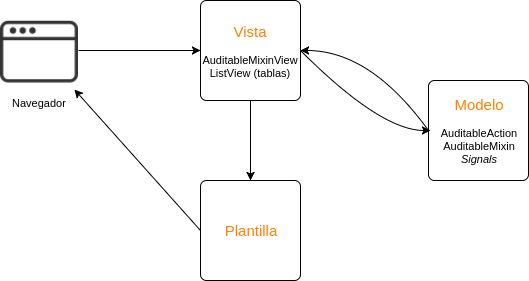
\includegraphics[width=0.7\textwidth]{Core.png}
\caption{Estructura del módulo \textit{Core} en el patrón MVT (creación propia).}
\label{fig:figura6.6}
\end{figure}

\subsubsection{Integración continua}

Luego de haber terminado gran parte del módulo \textit{Core}, se prosiguió a instalar Jenkins. Para esto, se ingresó al terminal de la computadora, se agregó el repositorio de la herramienta y se instaló.\\

Una vez realizado esto, el pasante ingresó, mediante la interfaz gráfica, al sistema de integración continua para configurar el repositorio del proyecto, ejecutando los siguientes pasos:

\begin{enumerate}
    \item Instalar el \textit{plugin} de Git en Jenkins.
    \item Agregar las credenciales de Git del pasante (usuario y contraseña) en el sitio administrador. De esta manera quedan almacenadas dentro de Jenkins para futuras acciones que las requieran.
    \item Incluir una “nueva tarea” para crear un nuevo proyecto.
    \item Clonar el repositorio, ingresando a la sección de  “Configuración” del proyecto creado y se proporcionó el enlace HTTPS. La herramienta permite seleccionar una rama específica de la cual hacer \textit{pull}; se escogió la rama "develop".
    \item En la configuración del proyecto, agregar la ejecución de un \textit{script} de shell luego de hacer \textit{pull} del repositorio para desplegar el proyecto.
\end{enumerate}

El pasante creó un \textit{script} que permite instalar el ambiente virtual y los \textit{plugins} necesarios para que el proyecto pueda ejecutarse, migrar la base de datos y ejecutar las pruebas. Esto es lo mínimo requerido por la HU. Adicionalmente, construyó otro \textit{script} que automatiza el empaquetamiento de la librería, el cual podría incluirse en el despliegue de la librería. \\

Por último, se probó la configuración de Jenkins mediante la interfaz. El pasante utilizó el botón de “build” y comprobó en la consola de la herramienta que se había descargado la información más reciente de la rama "develop" y que se había ejecutado el \textit{script} exitosamente. \\

Con el uso de Jenkins, se puede llevar el control de los despliegues de la librería y, en caso de que alguno falle, se puede detectar rápidamente verificando el estado del "build". De esta manera, gran parte del tiempo, la librería está disponible para la empresa y pueden verificar que sea estable sin necesidad de descargarla y probarla. \\

El comportamiento logrado con el \textit{script} mencionado anteriormente, no evita que en el repositorio exista una versión inestable, puesto que el “build” se efectúa luego de que los cambios han sido incluidos en el repositorio. Es por esta razón que el pasante decidió investigar sobre posibilidad de evitar que se incluya código que no pase las pruebas. \\

Dado que se utilizó Gitlab, se investigó sobre la configuración de Jenkins con este y se encontró que existe un \textit{plugin} que permite la integración de ambos sistemas. El pasante procedió a instalarlo, realizando las siguientes configuraciones sobre ambos sistemas:

\begin{itemize}
    \item En Gitlab, fue necesario generar un identificador único llamado “Gitlab API Token” creado para cada usuario. Adicionalmente, se debe crear un “Webhook” con el URL en el que está instalado Jenkins que incluye el proyecto en cuestión.
    \item En Jenkins, se utiliza el “Gitlab API Token” como credencial para conectarse con Gitlab. Luego, se procede a configurar el proyecto. En la sección de “Configuración”, el \textit{plugin}, agrega una nueva opción para accionar el empaquetamiento cuando ocurra un evento en Gitlab. En particular, el evento de \textit{push}.
\end{itemize}


Para crear el “Webhook”, era indispensable instalar Jenkins en un servidor de la empresa, para que el URL mencionado pueda accederse desde Gitlab. No obstante, el líder técnico consideró que no era necesario el comportamiento adicional descrito, así que se descartó.\\

El pasante dejó una documentación detallada acerca del proceso llevado a cabo para referencias futuras de algún otro miembro de la empresa, así como de la integración con Gitlab. Con esto, se pueden replicar fácilmente los pasos e instalar Jenkins en un servidor de la compañía e incluir otros proyectos, además de esta pasantía.

\subsubsection{Pruebas del módulo \textit{Core}}

Para el módulo Core, se generaron veintidós (22) casos de prueba automatizadas utilizando Pytest (ver Apéndice F). Dentro de estas pruebas, Once (11) consistían en validar el funcionamiento del "AuditableMixin", verificando que se guardara apropiadamente todos los campos la traza de auditoría. \\

Dentro del módulo de pruebas de la librería se agregaron cuatro (4) modelos con las relaciones mostradas en la figura 6.6, que sólo existen cuando se crean las pruebas. Al inicializar la ejecución de los casos, se efectúa una migración de la base de datos, que permite a estos modelos ser incluidos en el esquema. Estos, poseen relaciones suficientemente complejas para poder realizar casos de pruebas con uno-a-uno, uno-a-muchos y muchos-a-muchos.

\begin{figure}[h]
\centering
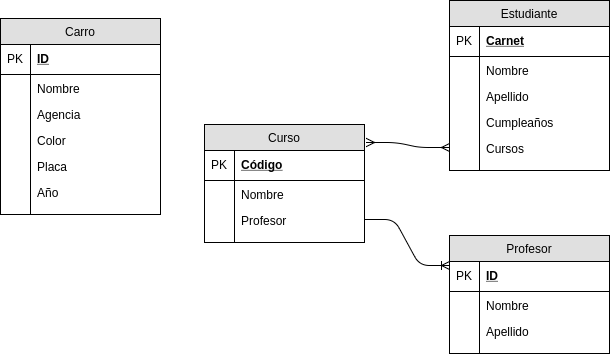
\includegraphics[width=0.7\textwidth]{Test_ER.png}
\caption{Modelo Entidad-Relación de la base de datos de prueba (creación propia).}
\label{fig:figura6.8}
\end{figure}


Antes de que comiencen a ejecutarse las pruebas, se precargan los registros con un \textit{Fixture} que utiliza el formato JSON.  Estos están escritos siguiendo la estructura de los \textit{serializers}; contienen la clave primaria, el modelo al que pertenece y el valor de cada campo como muestra la figura 6.9. Luego, se configuró Pytest para que utilizara el comando de Django “loaddata” y así, cargar el \textit{Fixture}. La base de datos es desechada al finalizar la ejecución.

\begin{figure}[h]
\centering
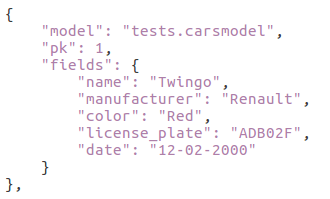
\includegraphics[width=0.6\textwidth]{Fixture.png}
\caption{Ejemplo del formato JSON para cargar un \textit{Fixture} (creación propia).}
\label{fig:figura6.8}
\end{figure}

De estos casos de prueba, se encontró que fallaron dos, debido a que el \textit{serializer} no excluía los campos “ManyToManyField”. Se corrigió el código según lo explicado en la sección sobre \textit{serializers}, y se obtuvo que todas las pruebas fueron exitosas.\\

Once de los casos de pruebas están dedicados a probar el "AuditableMixinView" para verificar que el usuario se agregue correctamente. Se configuró "RequestFactory" para simular un \textit{request} que solicitara un URL particular. De esta manera, se pueden probar las vista como se haría con cualquier otra función; con una entrada fija y una salida esperada, sin inspeccionar el contexto de la petición.\\

Todas estas pruebas resultaron exitosas exceptuando el caso C04-P06 (ver Apéndice F) puesto que al eliminar un modelo no-auditable con una referencia a otro que sí lo es, no se realiza la llamada a la función de la vista del modelo auditable. Por esta razón, no se almacena el usuario en estos registros. Esto fue documentado y se aceptó este pequeño error puesto que se conserva la integridad del sistema de auditorías.\\

Una vez terminada las pruebas unitarias y de integración, el módulo \textit{Core} cumple todos los requisitos del cliente, incluyendo el servidor de Integración Continua. De esta manera, se alcanzan los objetivos planteados.

\subsubsection{Permisología}

Con relación a la permisología de las auditorías, la HU C11 (ver Apéndice B) especifica que se desea contar con un sistema de autenticación (login) y que cada usuario autenticado posea un conjunto de permisos asociados. Estos, permitirán restringir ciertas acciones dentro de las auditorías, en particular visualizar listados. \\

Para crear el sistema de autenticación, se quería crear un modelo de usuarios para la librería. No obstante, al pasante investigar sobre esto, encontró que la documentación de Django indica que los \textit{plugins} no deben crear su propio modelo de usuarios. Debido a que podría generar conflictos con la aplicación que lo instale. Por consiguiente, se descartó la HU relacionada con la autenticación (C11.1). \\

Tomando en cuenta esto, se sugirió realizar un módulo de Permisología que incluyera, tanto las restricciones de los listados, como los de generación de reportes (PDF y CSV).\\

Dado que la implementación de este módulo no se encontraba en el objetivo de la pasantía, se decidió no incluirlo para esta versión de la librería. Sin embargo, el pasante decidió realizar el diseño del mismo con la intención de que sirva de referencia. \\

Este módulo también sería un microservicio, como Estadísticas y Reportes, que incluya permisos básicos y le brinde facilidades para generar nuevos permisos. Para restringir una funcionalidad específica, se utilizaría el mismo patrón de desarrollo del resto de la librería; ofrecer un \textit{mixin} que encapsule el comportamiento. Para obtener mayor detalle sobre el módulo de Permisología.

\subsubsection{Análisis de desempeño}

\subsubsection{Prototipo de tabla de auditorías descentralizada}

\subsection{Construcción del módulo Estadísticas}

En esta sección, se explica el desarrollo de módulo de Estadísticas; cómo se generaron los filtros, cálculos y gráficos necesarios, para presentar al usuario final la información recopilada por el módulo \textit{Core}.

\subsubsection{Creación del  formulario de filtros}

Para cumplir con las HU que se refieren al filtrado de los registros de auditoría, se procedió a crear un formulario. Inicialmente, se incluyeron aquellos campos relacionados con el rango de tiempo. De esta manera se puede construir el flujo de datos, básico, sin preocuparse por el resto de los filtros. Es importante destacar que ninguno de los campos es requerido y si no se selecciona, se obtiene toda la información.\\

Para crear los campos fecha de inicio, hora de inicio, fecha de fin y hora de fin; se aprovecharon los tipos “DateField” y “TimeField” de Django. Estos manejan la validación del formato de los valores ingresados y, en caso de ser correctos, procede a convertirlos en un objeto "datetime" de Python para facilitar su manipulación. Aunque Django posee un campo "DateTimeField", en el que se puede obtener tanto la fecha como la hora, se decidió mantener estos campos separados, para tener completo control sobre los validadores y rellenar la información no requerida. \\

El método “clean()” del formulario fue sobreescrito para manejar la lógica de los validadores y evitar el envío de un formulario incorrecto que pueda generar una excepción. Este método se encarga de:

\begin{itemize}
    \item Validar que la fecha de inicio no sea mayor que la de fin, tomando en cuenta la hora.
    \item Validar que la fecha de fin no sea mayor a la actual, tomando en cuenta la hora.
    \item Arrojar un error en el formulario cuando se coloca la hora (de fin o inicio) pero no la fecha relacionada. Este caso es muy importante puesto que no se puede filtrar únicamente con las horas porque generaría un error en el \textit{query}.
    \item En caso de que no sea ingresado, rellenar el campo de la hora de inicio con el valor 00:00.
    \item En caso de que no sea ingresado, rellenar el campo de la hora de inicio con el valor 23:59.
\end{itemize}


Una vez estructurado el formulario con el rango de tiempo, se prosiguió a armar el \textit{query} asociado. Para esto, se utilizó la vista prefabricada del \textit{framework} "ListView", que maneja toda la lógica de listar objetos utilizando un \textit{queryset} particular. La vista resultante se denominó "StatisticsView". Este \textit{queryset}  se configuró para que obtuviese todos los resultados de la tabla de auditorías, no obstante, el programador puede cambiar este atributo.\\

El formulario se incluye en una vista adicional llamada "FilterView" que hereda "StatisticsView". De esta manera, en el código se distingue fácilmente la lógica relacionada a los filtros y la relacionada con los gráficos. En "FilterView", se colocó el formulario en el contexto y si el mismo es válido, se procede a llamar a la función "build\_filters". Esta función, añade nuevos filtros al \textit{queryset} inicial, según los valores enviados en el formulario a través del método POST. \\

\begin{figure}[h]
\centering
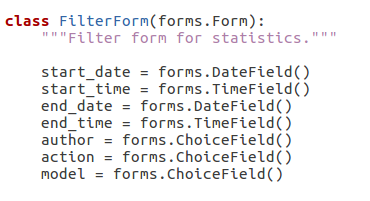
\includegraphics[width=0.6\textwidth]{form_filtros.png}
\caption{Estructura del formulario de filtros (creación propia).}
\label{fig:figura6.9}
\end{figure}


Es importante destacar que el \textit{framework} maneja los \textit{queries} de manera "lazy", lo que quiere decir que no serán evaluadas hasta que realmente sean necesarias. Este comportamiento permite filtrar el \textit{queryset} inicial tantas veces como indique el formulario, sin necesidad de cargar todos los objetos en memoria ni aumentar el tiempo de respuesta del usuario.\\

También se agregaron tres botones que permiten agilizar el envío del formulario cuando se desea filtrar por la fecha, mes o año actual. Estos botones rellenan los campos de fecha según sea el caso, haciendo uso de funciones de JavaScript.\\

Una vez creada la estructura que permite filtrar por rango de tiempo, se procedió a agregar al formulario, los campos “action”, “model” y “author” para filtrar por tipo de acción, modelo y autor respectivamente. Con cada uno de ellos, se repitió el proceso descrito anteriormente.

\subsubsection{Cálculos estadísticos}

Luego de obtener el \textit{queryset} filtrado, se procedió a construir los cálculos estadísticos indicados por los requerimientos: el promedio, máximo, mínimo y total de elementos. Para esto, se procesa el \textit{queryset} creando un diccionario, llamado "stats",  cuya clave es el día en que fue realizada la operación y su valor es la cantidad de transacciones en ese día.\\

\begin{figure}[h]
\centering
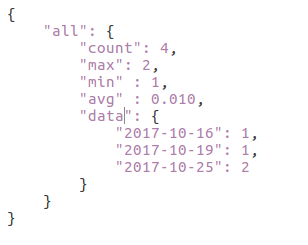
\includegraphics[width=0.5\textwidth]{stats.png}
\caption{Ejemplo de “stats” (creación propia).}
\label{fig:figura6.10}
\end{figure}

En el formulario, se creó la función "days\_elapsed" para obtener la cantidad de días transcurridos entre la fecha de inicio y la de fin. Este valor se utiliza para calcular el promedio apropiadamente, dividiendo el total de operaciones entre la cantidad de días transcurridos. Si no se provee fecha de inicio, se toma la fecha del primer objeto en la tabla de auditorías para calcular la diferencia de fechas.\\

Para calcular el porcentaje de crecimiento, en "build\_filters" se determina la cantidad de registros que ocurrieron antes de la fecha de inicio ingresada en el formulario. Este valor, denominado "offset", se utiliza para conocer cuántas auditorías se registraron en el periodo anterior. El porcentaje de crecimiento se calcula restando el valor de periodo anterior con el actual, y dividiéndolos entre la cantidad total de modelos.\\

En cuanto a la cantidad de modelos auditables, se utilizó la función "get\_models" de Django que retorna una lista de todos los modelos de la aplicación. Cada modelo es representado por un objeto que incluye su clase, con el cual se puede contar cuántos heredan el "AuditableMixin". Siguiendo este mismo procedimiento se puede determinar el porcentaje de cobertura de la librería, dividiendo la cantidad de modelos auditables entre el total de modelos.\\

Todos los cálculos de estadísticas se colocan en el contexto de la vista "StatisticsView" para que puedan ser utilizados en las plantillas.

\subsubsection{Construcción de gráficos}

Antes de procesar los datos necesarios para crear un gráfico, se investigó en profundidad las funcionalidades que provee Amcharts. Este \textit{plugin}, requiere crear un elemento en HTML con la etiqueta "<div>", que posea un identificador único (atributo id) con el que se pueda referenciar para construir el gráfico con JavaScript. Para esto, se utiliza la función "Amcharts.makeChart" pasando como parámetros el identificador y un objeto con las opciones para crearlo.\\

Los gráficos de Amcharts son altamente configurables, pues cuentan con una gran cantidad de opciones que permiten crear comportamientos complejos. Entre estas opciones se destacan:

\begin{itemize}
    \item dataProvider: datos para mostrar el gráfico en formato JSON. Puede contener cualquier cantidad de campos y se puede utilizar cualquier.
    \item type: tipo de gráfico. Los posibles valores de esta opción son: “serial", “pie", “xy", “radar", “funnel", “gauge", “map", “gantt" y “stock".
    \item theme: tema o estilo del gráfico. Amcharts posee unos temas propios creados en JavaScript, algunos de estos son "chalk" "black" "light".
    \item balloon: crea los mensajes que aparece al posicionar el cursor sobre los ítems del gráfico. Amcharts crea automáticamente la información que aparece, sólo se necesita ajustar la apariencia.
    \item graphs: crea la visualización de los datos en los siguientes subtipos de gráfico: “line”, “column”, “step line”, “smoothed line”, “olhc” y “candlestick”. Cuenta con varias opciones de personalización, incluyendo la posibilidad de modificar la información mostrada en el “balloon”
    \item legend: leyenda del gráfico en cuestión.
    \item export: habilita un menú que permite exportar los datos en diferentes formatos.
    \item responsive: ajusta el tamaño del gráfico dependiendo de la pantalla.
\end{itemize}


Para construir los gráficos con Amcharts, se creó una clase llamada "ChartData" que encapsula toda la lógica necesaria para obtener la información relacionada con él. La clase cuenta con atributos como el identificador, tipo, tema, y los datos. Este último, denominado "data", se inicializa con el resultado de procesar "stats", y convertirlo en un objeto JSON. De esta manera, puede ser utilizado como "dataProvider". La mencionada clase puede ser heredada por el programador y ampliada para ajustarlo a sus necesidades.\\

La clase "ChartData" es usada para crear una variable en el contexto de la vista "StatisticsView" que posea toda la información, y así, pueda ser utilizada en la plantilla. En la vista se incluyen seis gráficos:

\begin{itemize}
    \item Gráfico de línea con la evolución de las auditoría.
    \item Gráficos de torta con la comparación entre cantidad de operaciones por autor, por modelo y por acción.
    \item Gráfico de columnas apiladas con la comparación de cada operación realizada por cada usuario.
    \item Gráfico de columnas apiladas con la comparación de cada operación realizada sobre cada modelo.
\end{itemize}


\subsection{Plantillas del módulo Estadísticas}

Dado que el sistema en cuestión es una librería, es sumamente importante que las plantillas generadas sean fáciles de utilizar y personalizar por el programador que las utilice. Por esta razón, se crearon varias plantillas que pueden agregarse en el sistema "Host" haciendo uso de la etiqueta  "include". Esta etiqueta permite a Django, cargar y mostrar un plantilla utilizando el contexto e incluso se puede pasar parámetros para incluir nuevos valores de variable en el contexto.\\

Entre las plantillas creadas, la principal es "turpial\_statistics.html" que incluye varios componentes:

\begin{itemize}
    \item El formulario del filtro.
    \item Todos los cálculos estadísticos.
    \item Gráfico de línea con la evolución de las auditoría.
    \item Gráficos de torta con la comparación entre cantidad de operaciones por autor, por modelo y por acción.
    \item Gráfico de columnas apiladas con la comparación de cada operación realizada por cada usuario.
    \item Gráfico de columnas apiladas con la comparación de cada operación realizada sobre cada modelo.
\end{itemize}

Si el programador desea una plantilla con toda la información relacionada con las estadísticas puede incluir esta plantilla en las propias.\\

En cuanto a los gráficos, se observó que la creación de cada uno era similar; por lo que se decidió fabricar una plantilla reutilizable que recibe como parámetro el objeto de la clase "ChartData". Con esto, se le ofrece al programador una manera sencilla de crear gráficos de Amcharts. Además, es utilizado en "turpial\_statistics.html" para generar los gráficos que ofrece. \\

Esta idea fue aplicada a los cálculos estadísticos con las plantillas "turpial\_cards.html" y "turpia\_card\_stats.html". La primera presenta la información general relacionada con la librería, como la cantidad de modelos auditables, porcentaje de cobertura y de crecimiento. La segunda, muestra las estadísticas relacionada con la cantidad de registros auditables (promedio, máximo, mínimo, total). El programador puede utilizar cada plantilla para presentar la información como mejor le convenga en caso "turpial\_statistics.html" no se ajusta a sus necesidades.\\

Todas las plantillas utilizan Bootstrap para mostrar la información, dado que la empresa posee como estándar de desarrollo, este \textit{framework}.\\

Adicionalmente, se creó un tema propio para los gráficos ("turpial.js"), aprovechando las facilidades que ofrece Amcharts. En este tema, se configuraron los colores de los gráficos, el estilo de las leyendas, el tamaño de las letras entre otros.\\

El programador también puede crear su propio tema, utilizando el atributo del "StatisticsView" llamado "chart\_theme". Este  requiere un diccionario con el nombre del tema y su ubicación en el proyecto (dirección). La dirección fue incluida dado que el tema debe cargarse después que el JavaScript principal de Amcharts pero antes de generar el gráfico o no estará disponible. El valor de la variable "chart\_theme" se utiliza en el atributo del tema en la clase "ChartData".\\


\begin{figure}[h]
\centering
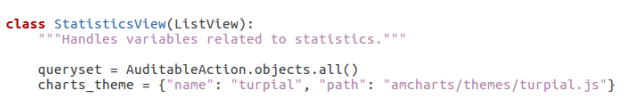
\includegraphics[width=\textwidth]{StatisticsView.png}
\caption{ Definición de “StatisticsView”  incluyendo el campo “charts\_theme” (creación propia).}
\label{fig:figura6.11}
\end{figure}


Para el resto de los estilos, el programador tiene completa libertad de sobreescribirlo al cambiar el estilo de Bootstrap como lo indican.\\


\begin{figure}[h]
\centering
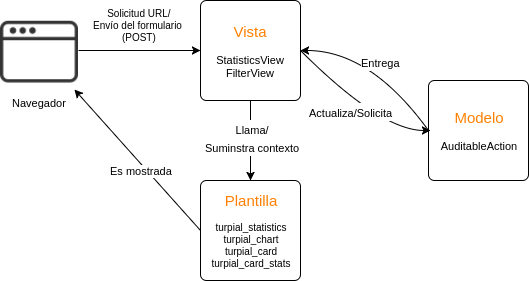
\includegraphics[width=0.7\textwidth]{Estadisticas.png}
\caption{ Estructura del módulo de Estadísticas (creación propia).}
\label{fig:figura6.11}
\end{figure}

Luego de culminar las plantillas, se posee un módulo de Estadísticas que cumple con todos los requerimientos establecidos. En la figura 6.11 se muestra la estructura final del módulo de Estadísticas y en dónde se ubica cada función del mismo.

\subsubsection{Pruebas del módulo Estadísticas}

Para el módulo de estadísticas se escribieron 106 casos de prueba, utilizando los mismos modelos que en el módulo \textit{Core} y el mismo \textit{Fixture}. De estos casos, 73 corresponden al formulario de filtros y 33 a los cálculos estadísticos en la vista “StatisticsView". \\

Las pruebas del formulario se enfocan en determinar si es válido, y si lo es, proceder a filtrar el queryset inicial según los valores provistos. Para comparar que los resultados obtenidos en el \textit{queryset} son los esperados, se utilizó la función “filter" de Python sobre la lista de todos los elementos de la tabla. También, se incluyeron los casos de pruebas en el que el formulario es inválido, en ellos se verifica que ocurra una excepción que incluya un mensaje de error que notifique al usuario. Esto permite asegurar que los filtros funcionan correctamente. Al ejecutar estas pruebas, se obtuvo que todas fueron exitosas.\\

Para los cálculos estadísticos se deben probar las funciones que entregan estos resultados, haciendo una solicitud POST al URL que llama a la vista “FilterView". Para esto, se utilizó “Client()" una clase de Django que permite enviar la petición, simulando el navegador. De esta manera se puede inspeccionar el contexto e incluso el HTML de la respuesta, y así constatar que los valores son los esperados. \\

Al ejecutar estas pruebas fallaban todas, excepto las que obtenían los resultados sin filtrar. Esto sucedió debido a que no se enviaban correctamente los datos del formulario que están relacionados con el tiempo. Para corregir el error, todos los valores fueron convertidos en \textit{string}. \\

Luego, fallaron las relacionadas con el filtro de “acción". No se estaba calculando el “offset" en este caso, por lo que el porcentaje de crecimiento era incorrecto. Se corrigió el código y las pruebas fueron exitosas.\\

Otro problema que surgió fue que, como el promedio cambia a medida que pasan los días, cuando no se envía la fecha de fin las pruebas comenzaron a fallar a medida que avanzaron los días. Para lidiar con esto, se creó una función, en lugar de colocar un valor fijo con el cual comparar el promedio como se estaba haciendo con el resto de las estadísticas. Esta función divide la cantidad de registros esperados entre días transcurridos para calcular el promedio. Los días transcurridos fueron obtenidos con la función “days\_elapsed". Luego se obtuvo que las pruebas fueron exitosas.\\

Finalmente, se crearon casos de pruebas en los que se genera un modelo al momento de ejecutar el caso en particular. Con la intención de validar que se calculan correctamente la cantidad de modelos auditables y el porcentaje de cobertura. Estas pruebas resultaron exitosas.

\section{Fase de transición}

En esta sección se explica el proceso de integración de la librería en el proyecto Turpial Calendar, los errores encontrados y sus correcciones. Así como, la puesta en producción de ese sistema. Este proceso duró una semana.

\subsection{Integración de la librería con Turpial Calendar}

Antes de iniciar el proceso de integración, se descargó el proyecto Turpial Calendar y se instalaron los paquetes de los cual depende. Este proyecto utiliza Django 1.11 y MySQL. \\

A continuación, se instaló la librería Auditorías Turpial (turpial\_auditor); utilizando la facilidad que ofrece PIP para esto, a través del enlace de un repositorio. Este proceso se repitió para Auditorías Turpial UI (turpial\_auditor\_ui).\\

Con respecto a la configuración de las librerías, se siguió paso a paso la documentación correspondiente. En primer lugar, se incluyeron en “INSTALLED\_APPS" los módulos necesarios para registrar las auditorías y para visualizar las estadísticas. Luego, agregaron modelos auditables utilizando el \textit{mixin} para esto. Los modelos que presentan auditorías son: Eventos, Proyectos, Empleado y Categoría (de un calendario).\\

De estos modelos, se ubicaron las vistas que permiten crear y eliminarlos y se incluyó el \textit{mixin} para agregar el usuario en la traza de auditorías, “AuditableMixinView".\\

Después, se incluyó un URL en Turpial Calendar que llamase al “FilterView” y que permitiera ver la plantilla de estadísticas. Se repitió este proceso para crear otra plantilla que utilice los estilos de Turpial Calendar y se reorganice la información de otra manera para probar esta funcionalidad.\\

\textbf{Errores encontrados}  Se ejecutó el proyecto y se intentó crear un evento en el calendario para verificar que las auditorías se estaban realizando. Sin embargo, al tratar de enviar el formulario ocurrió una excepción relacionada con el campo “ForeignKey”. Django incluye en los modelos, un campo oculto para realizar una referencia “hacia atrás” para obtener el modelo que guarda una relación con este. Al excluir los campos muchos-a-muchos en el serializer se utiliza una función que permite determinar cuales son y se accede al nombre de dicho atributo. Este campo oculto, no posee la función que accede al nombre y esto ocasionaba la falla.\\

Una vez detectado el error, se corrigió y se constató que el \textit{Core} funcionaba como se esperaba. Luego, se escribieron tres nuevas pruebas para validar que este error fue solventado. Para esto, se agregaron dos nuevas tablas en la base de datos de prueba: Compañía y Persona, como se muestra en la figura 6.13. Estas pruebas fueron exitosas.\\


\begin{figure}[h]
\centering
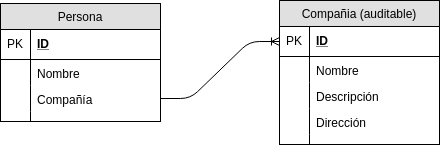
\includegraphics[width=0.6\textwidth]{New_Test_ER.png}
\caption{ Diagrama Entidad-Relación de los nuevos modelos en las pruebas (creación propia).}
\label{fig:figura6.13}
\end{figure}


En el módulo de Estadísticas se encontró un pequeño error en el cálculo de la cantidad de días transcurridos entre la fecha de inicio y la de fin. Cuando no se envía la fecha de inicio en el formulario, se escogía la fecha del primero objeto auditable. Sin embargo, si este es borrado de la base de datos, no se obtenía ninguna fecha para realizar el cálculo. Esto se solucionó utilizando el mismo \textit{queryset} ya filtrado y obteniendo el primer registro que posee.

\subsection{Puesta en producción}

Finalizado el proceso de integración, se prosiguió a poner el proyecto Turpial Calendar en el servidor de Turpial Development, Webfaction. Para esto, se ingresó a este sistema y se creó un sitio web, agregando el dominio en el que estaría disponible el proyecto. Después, se configuró el tipo de aplicación (Django), se creó la base de datos con su respectivo usuario y contraseña y se migró. \\

Para clonar el repositorio de Turpial Calendar, se ingresó mediante el protocolo SSH al servidor y luego se creó el ambiente virtual del proyecto. Se instalaron las dependencias y las librerías turpial\_auditor y turpial\_auditor\_ui desde su respectivos repositorios.\\

A continuación, se configuró el servidor web, Apache. Se agregó un nombre de servidor, un alias y una tarea para activar el servidor (\textit{daemon}). \\

Finalmente, se comprobó que el sistema funcionara correctamente, incluyendo las librerías y todas las funciones relacionadas con ellas.
